\section{Selección de componentes}
Se decidieron una serie de requerimientos simplificados para el prototipo a fin de poder seleccionar los componentes y el diseño adecuados.
\begin{itemize}
    \item \textbf{Dimensiones:} 60cm x 60cm x60cm
    
    \item \textbf{Peso total:} 25Kg

    \item \textbf{Alcance efectivo:} 50m
    
    \item \textbf{Velocidad Máxima:} 3km/h
    
    %\item \textbf{Autonomia minima:} 6hs
\end{itemize}
\subsection{Ruedas}
Se eligieron ruedas neumáticas 4.10/3.5-4 para 80 kg de carga, estas ruedas presentan buena tracción en terrenos difíciles y una buena capacidad de carga.

\begin{figure}[H]
\centering
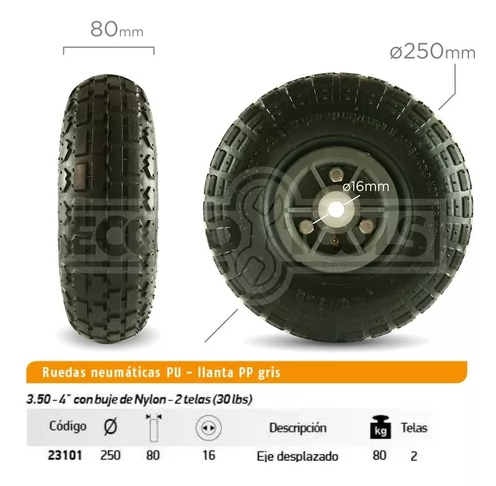
\includegraphics[width=.75\textwidth]{Figures/rueda.png}
\label{fig:rueda}
\caption{Datos de las ruedas elegidas}
\end{figure}

Al conocer el diámetro de las ruedas se pueden calcular el torque y las rpm de los motores.


\subsection{motores de tracción}

Para los motores de tracción de opto por motores PGM36-555, que son motores de 24V DC con reductor satelital, estos motores entregan 24Kgf/cm a 45rpm (58rpm en vacio) con un consumo de 0.7A, y un torque maximo de 80Kgf/cm con un consumo de 7.5A.

Con las ruedas previamente seleccionadas se puede calcular la velocidad robot

\begin{align*}
RPM &= 45 \\
D &= 0{,}25\,\text{m} \\
C &= \pi \cdot D = \pi \cdot 0{,}25 \approx 0{,}7854\,\text{m} \\
\end{align*}

Entonces la velocidad se calcula como:

\begin{align*}
v_{\text{m/s}} &= \frac{RPM \cdot C}{60} = \frac{45 \cdot 0{,}7854}{60} \approx 0{,}589\,\text{m/s} \approx 2{,}12\,\text{km/h}
\end{align*}

\subsection{Motores de la torreta}

Para los dos ejes de la torreta se opto por motores stepper por su capacidad de mantener la posición al mantener energizadas las bobinas.

Para el eje X se opto por un motor tipo nema 17 de aproximadamente 2.6Kg/cm de torque de holding.

Para el eje Y, ya que este tiene que sostener el peso del arma se opto por un motor tipo nema 23 con reductor tipo sinfin y corona.

\subsection{Drivers de motor}

Una vez definidos los motores se buscaron los drivers para estos.

Para los motores de traccion se seleccionaron modulos puente H basados en BTS7960 ya que soportan tenciones entre 5.5V y 27V y corrientes de hasta 43A.

Para el motor nema 17 del eje X se opto por el driver A4988

El motor nema 23 del eje Y ya poseia su propio driver TB6600

\subsection{Interfaz con la PC}

Como el procesamiento sera realizado en la pc y la interfaz solo cumple la tarea de traducir las ordenes de esta a los drivers de motor se opto por una placa de desarrollo arduino nano, ya que esta cuenta con un puerto serie para conectarse a la pc y suficientes pines I/O para controlar todos los motores necesarios.

\begin{figure}[H]
\centering
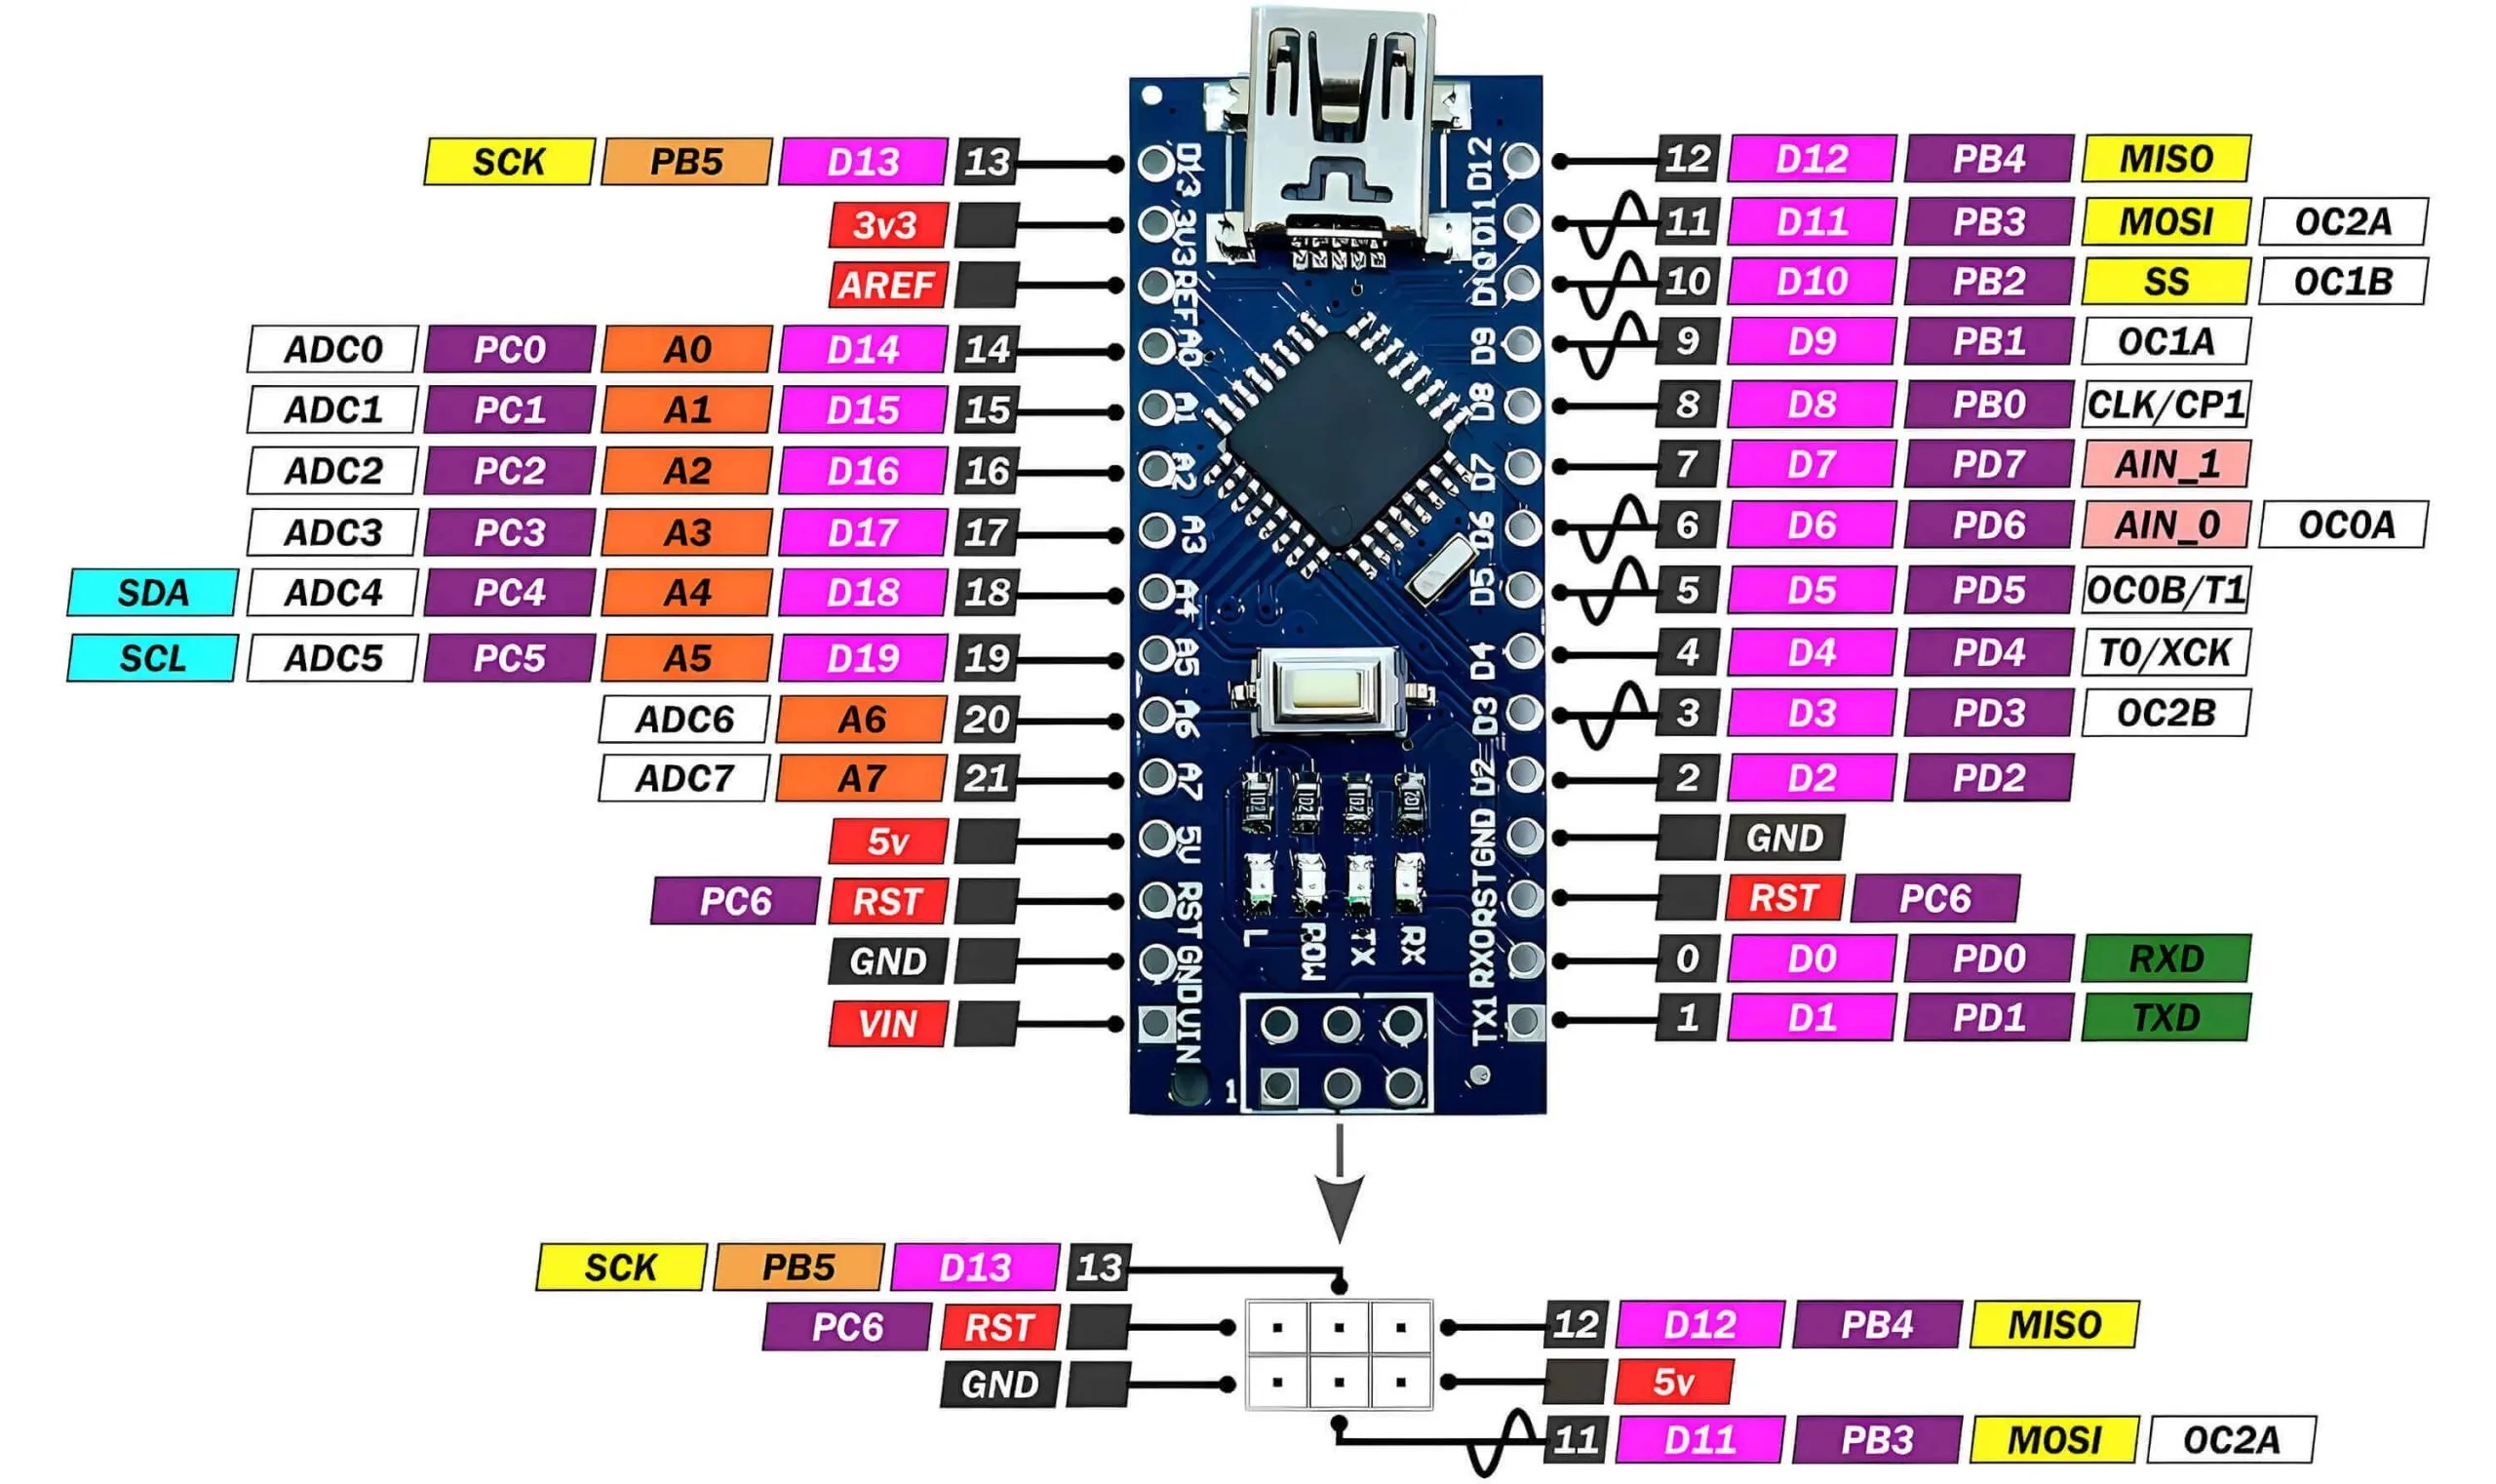
\includegraphics[width=1\textwidth]{Figures/arduino.jpg}
\label{fig:arduino}
\caption{Pinout del Arduino nano}
\end{figure}

\subsection{Baterias}

Ya que los motores serian alimentados a 24v se opto por usar baterias recargables de gel de 12V y 7Ah puestas en serie para obtener los 24V
